% objectives.tex
\section{Research Objectives}
\label{objectives}
%
The objective of this project is to automatically map a given application requirements to physical hardware resources such that the application performance can be maintained in a highly consolidated environments. 

The virtualization layer will provide the framework to partition the available hardware resources and to isolate the performance interference between them\cite{}. 
The management layer will provide means to create a \emph{pool} of resources from cluster of heterogenous machines\cite{}, increasing the total amount of resources available for mapping. 
Live migration techniques\cite{} allow applications to be remaped based on the time varying demands and machine availbility. 
These mechanisms already exists in current virtulization infrastructure.
However, the mapping itself is still carried out manually decreasing the benefits of virtualization and explosing the system to the human error. 

To achieve our objective, the system must be aware of the workload changes, remap the resources and ensure that remaping satisfies the requirements of all active applications.
A significant progress has already been made to migrate virtual machines to load balance CPU and memory resources\cite{}.
However, correct IO performance prediction is a much harder problem due to the statefulness of the storage systems\cite{}.
Another problem is that virtualization fails to isolate the performance interference of consolidated IO workloads as well as it isolates the CPU, memory and network resources. 
Last problem is lack of mapping between the application requirements and the virtualized resources. 
The actual application requirements are typically not specified interms of resource usage. 
Instead they are typically determined by the end user demand it must satisfy.   
A mechanism to monitor and model the application performance behavor is the last requirement of this project. 

\subsection{Intellectual Merit of the Proposed Work}

Romano\cite{} project reveals that the workload and storage models are highly dependent for certain class of workloads. 
This confirms observations from other works~\cite{relative-fitness, benchmark}.  
%Whereas techniques based on independent models have been shown to have good average-case behavior, they work suffers from severe corner case model inaccuracies. 
%These can lead to expensive bad data movement recommendations. 
%Furthermore, the cost-benefit analysis in earlier work has largely ignored the time-series nature of the workload interference into account, further eroding accuracy.
Early efforts to automatically manage storage resources in a virtualized environment such as \emph{VectorDot}~\cite{vectordot} ignored the workload and simply concentrated on utilization of each storage system. 
A workload from the over-utilized device is simply migrated over to less utilized device. 
This approach would fail to work in a heterogeneous storage environment since the resulting performance is unknown.
Furthermore, the goal is not to simply ensure that no storage system suffers from over-utilization but to ensure that no workload suffers from degraded performance. 

Other work has focused on highly accurate latency prediction of workloads across storage devices but this has come at the cost of practicality by requiring extensive off-line experimentation and modeling. 
For instance, Wang et al.~\cite{relative-fitness} developed CART models off-line to develop workload-storage models. 
In contrast to their work, we plan to learn storage behavior quickly using online calibration without resorting to intrusive off-line methods.

\subsection{Impact on VMware}
%
In our previous work with VMware, we developed a storage performance modeling framework called Romano. 
This differs from previous model, Pesto\cite{}, currently in use by \emph{Virtual Center} product in that it identifies the key characteristics of workload that affects the performance (using ANOVA\cite{}).
The resulting accuracy is improved by 80\% allowing much more aggressive load balancing. 
\begin{figure}[t!]
\centering
\subfloat[Pesto]{\label{rdPesto}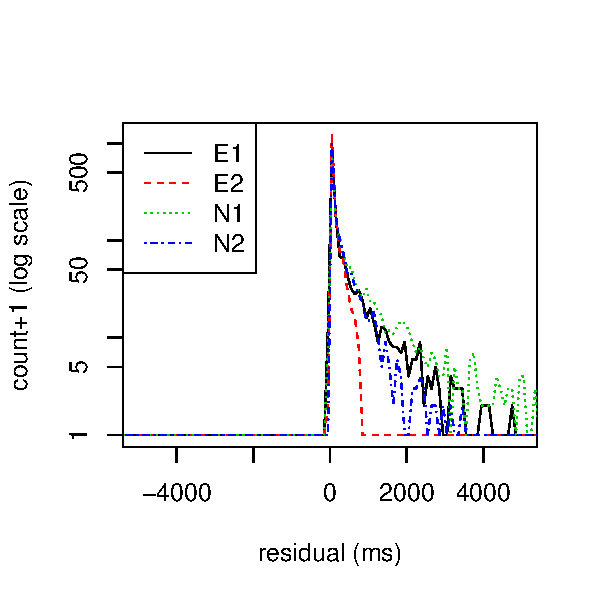
\includegraphics[width=0.4\columnwidth, clip, trim=0 0.5in 0.2in 0.7in]{error_hist_compare_pesto.pdf}}
\subfloat[Romano]{\label{rdRomano}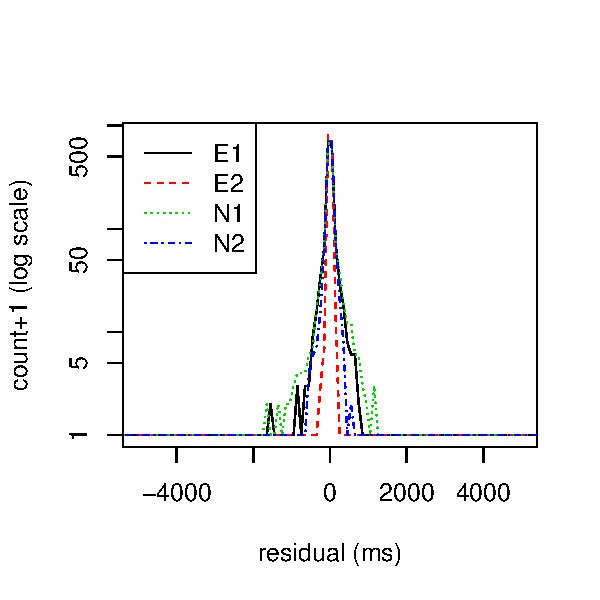
\includegraphics[width=0.4\columnwidth, clip, trim=0 0.5in 0.2in 0.7in]{error_hist_compare_kromano.pdf}}
\caption{Distribution of residuals($\epsilon$) for Pesto and Romano.
x-axis is the value of $\epsilon$ in $ms$.
y-axis is number of occurrences+1.
Addition of 1 was required to allow y-axis to be in log scale.
%The $\epsilon$ distribution does not changes widely for Romano indicating that the accuracy of Romano is less data store dependent. 
%Furthermore, Romano's $\epsilon$ are symmetric around 0, indicating that residuals are unbiased.
}
\label{residualDist}
\end{figure}
The residuals from both techniques are shown in Figure \ref{residualDist} for four different storage systems.
While this approach is very good at predicting a data store performance, it currently lacks the ability to predict the performance for each virtual disk when they are consolidated onto a single data store. 
By applying statstical inference on the effect of interference, we plan to derive each VM's IO performance without having to actually change the system state. 
This allows IT administrators to simulate their configuration changes in the large scale data centers without disrupting their operation. 

Furthermore, by allowing application level performance requirements to be mapped to VM level configurations, users can simply specify the desired behavior without having to worry about the VMware product details. 
